\documentclass[a4paper,norsk, 10pt]{article}
\usepackage[utf8]{inputenc}
\usepackage{verbatim}
\usepackage{listings}
\usepackage{graphicx}
\usepackage[norsk]{babel}
\usepackage{a4wide}
\usepackage{color}
\usepackage{amsmath}
\usepackage{float}
\usepackage{amssymb}
\usepackage[dvips]{epsfig}
\usepackage[toc,page]{appendix}
\usepackage[T1]{fontenc}
\usepackage{cite} % [2,3,4] --> [2--4]
\usepackage{shadow}
\usepackage{hyperref}
\usepackage{titling}
\usepackage{marvosym }
\usepackage{subcaption}
\usepackage[noabbrev]{cleveref}
\usepackage{cite}


\setlength{\droptitle}{-10em}   % This is your set screw

\setcounter{tocdepth}{2}

\lstset{language=c++}
\lstset{alsolanguage=[90]Fortran}
\lstset{alsolanguage=Python}
\lstset{basicstyle=\small}
\lstset{backgroundcolor=\color{white}}
\lstset{frame=single}
\lstset{stringstyle=\ttfamily}
\lstset{keywordstyle=\color{red}\bfseries}
\lstset{commentstyle=\itshape\color{blue}}
\lstset{showspaces=false}
\lstset{showstringspaces=false}
\lstset{showtabs=false}
\lstset{breaklines}
\title{FYS3140 Home exam}
\author{Kandidatnr. 15135}
\begin{document}
\maketitle

\section*{1)}

We have the differential equation

\begin{equation}
t^2 \frac{d^2u}{dt^2} - t\frac{du}{dt} + u = t
\end{equation}

This is on the form of a Euler-Cauchy equation, meaning that we can solve it by doing the change of variable:

$$
t = e^z, \qquad \frac{dz}{dt} = \frac{1}{t} \qquad (t>0)
$$
$$
t = -|t| = -e^z, \qquad \frac{dz}{dt} = \frac{1}{t} \qquad (t<0)
$$

From $\frac{dz}{dt} = \frac{1}{t}$ we see that $t \neq 0$. After the change of variable the differential equation takes the form

\begin{equation}
\frac{d^2u}{dz^2} + (-1 -1)\frac{du}{dz} + u = e^z
\label{eq:transformed_DE}
\end{equation}

So is a inhomogeneous 2. order ODE, and is easy to solve. We have to do it in 2 steps. We will first find the homogeneous solution $u_h$, and then a particular solution $u_p$. From these we can find the general solution.\\

$\underline{\mathbf{u_h}}$:\\

The homogeneous equation is:

$$
u'' - 2u' + u = 0
$$

Using the ansatz that the solution is on the form $e^{\lambda z}$ we get the characteristic polynomial:

$$
\lambda^2 -2\lambda + 1 = 0
$$

The solution(s) is

$$
\lambda = \frac{2 \pm \sqrt{4-4}}{2} = 1
$$

The characteristic polynomial has only one solution $\lambda = 1$, giving us the solution $u_1(z) = Ae^z$. But to span the entire solution space of the differential equation we need two linear independent solutions. From the variation of parameters we know that we can construct such an solution be multiplying the first solution by $z$, giving us $u_2(z) = Bze^z$. Since we now have two solutions we can write down the homogeneous solution:

\begin{equation}
u_h(z) = Ae^z + Bze^z
\end{equation}

We can now find a particular solution: \\

\newpage

$\underline{\mathbf{u_p}}$:\\

We now have to look at 

$$
u'' - 2u' + u = e^z
$$

We are going to make a 'guess' for the 	particular solution. We are going to make the guess that the solution is on the form $u_p = Q_n e^z$, where $Q_n$ is a polynomial of degree $n$. The particular solution can not be on the same form as the general solution, so it can not be on the form $e^z$ nor $ze^z$. The smartest guess is $Q_2 e^z$, and the easiest polynomial of degree 2 is $Cz^2$, so we are going to guess:

$$
u_p(z) = Cz^2e^z
$$ 

We need the derivatives:

$$
u_p' = C(2ze^z + z^2e^z), \qquad u_p'' = C(2e^z + 4ze^z + z^2e^z)
$$

We can so insert this back into the differential equation:

$$
u'' - 2u' + u = C(2e^z + 4ze^z +z^2e^z - 4ze^z - 2z^2e^z + z^2e^z) = e^z
$$

Most of the terms disappears, and we get:

$$
2Ce^z = e^z \Rightarrow C = \frac{1}{2}
$$

Giving us the particular solution

$$
u_p(z) = \frac{1}{2}z^2 e^z
$$

We now have all we need to find the general solution:

$$
u(z) = u_h(z) + u_p(z) = Ae^z + Bze^z + \frac{1}{2}z^2 e^z
$$

But this is only the solution for \eqref{eq:transformed_DE}. We need to change the variable back to the original variable. But since we can have both negative and positive $t$ we are going to use $|t|$ in the general solution. We use that

$$
z = \ln |t|
$$

We now get the correct general solution:

\begin{equation}
\underline{u(t) = \tilde{A}t + \tilde{B}t\ln |t| + \frac{1}{2}t \ln |t|^2}
\end{equation}


We can now apply the initial conditions $u(1) = 1$, $u(e) = 2e$:

$$
u(1) = \tilde{A} = 1 
$$
$$
u(e) = \tilde{A}e + \tilde{B}e + \frac{1}{2}e = 2e \Rightarrow \tilde{B} = \frac{1}{2}
$$

This gives us the final solution:

\begin{equation}
\underline{\underline{u(t) = t +\frac{1}{2}t\ln |t| + \frac{1}{2}t\ln |t|^2}}
\end{equation}
\newpage

\section*{2)}

\subsection*{a)}

We are going to evaluate 

$$
\bigg| \int_{\gamma} \frac{e^{3z}}{1+e^z} dz \bigg| 
$$

Where $\gamma$ is the straight line from $z = R$ to $z = R + 2\pi i$, where $R > 0$.\\

\begin{figure}[H]
\centering
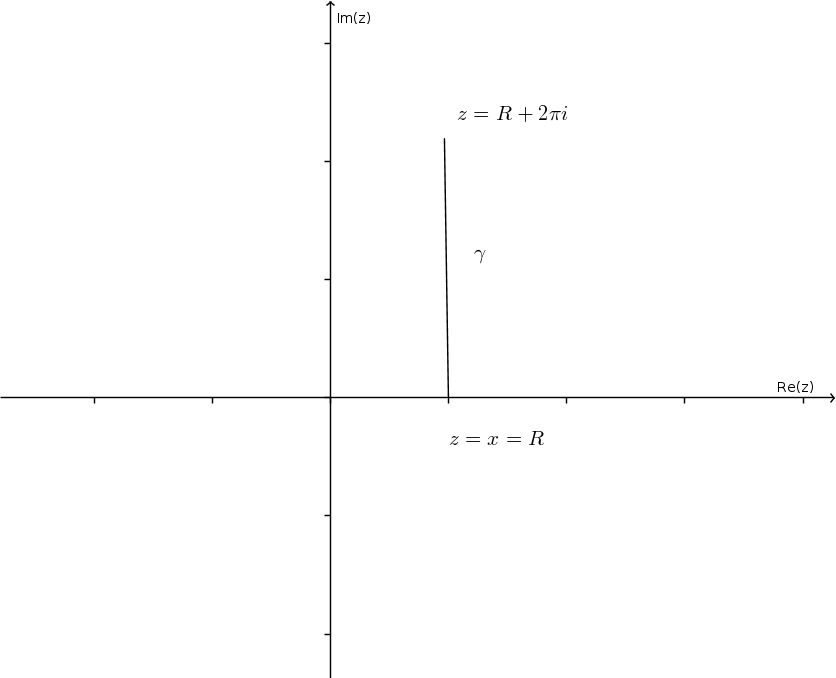
\includegraphics[scale=0.4]{2a.png}
\caption{The contour $\gamma$(suppose to be a straight line).}
\end{figure}

We know from upper bound estimates of contour integrals that:

$$
\bigg| \int_{\gamma} f(z) dz \bigg| \leq M l 
$$

Where $M = \max_{\gamma} |f(z)|$ and $l$ is the length of $\gamma$. First we are going to evaluate

$$
M = \max_{\gamma}\bigg|\frac{e^{3z}}{1+e^z}\bigg|
$$

First we look at the numerator. We want the numerator to become as large as possible. To do this we are going to parameterize the curve $\gamma = R + \theta i$, where $0\leq \theta \leq 2\pi$:

$$
\max_ {\gamma} |e^{3z}| = \max_ {\gamma} |e^{3(R + \theta i)}| = \max_ {\gamma} |e^{3R}e^{3\theta i}|=\max_ {\gamma} |e^{3R}||e^{3\theta i}|
$$

The term $e^{3\theta i}$ is just a rotation, meaning that $|e^{3\theta i}| = 1$. So:

\begin{equation}
\max_ {\gamma} |e^{3z}| = \max_ {\gamma} |e^{3R}| = e^{3R}
\label{eq:maxNum}
\end{equation}

We now look at the denominator. To get the whole expression to be as big as possible, we want the denominator to be as small as possible:

$$
\min_{\gamma} |1+ e^z| = \min_{\gamma}|e^z - (-1)| \geq \min_{\gamma}(|e^z| - 1) = e^R -1
$$

I used $|e^z| - 1$ instead of $1-|e^R|$ to make sure that the denominator is positive, since $R<0 \Leftrightarrow e^R > 1$. So now we have the maximum on the contour:

\begin{equation}
M = \frac{e^{3R}}{e^R - 1}
\label{eq:M}
\end{equation}

We can now look at the length $l$, which is the end point minus the starting point:

\begin{equation}
l = |(R + 2\pi i) - R | = |2\pi| = 2\pi
\label{eq:l}
\end{equation}

Combining \eqref{eq:M} and \eqref{eq:l}, we finally find that:

$$
\underline{\underline{\bigg| \int_{\gamma} \frac{e^{3z}}{1+e^z} dz \bigg| \leq M l = \frac{2\pi e^{3R}}{e^R-1}}}
$$




\subsection*{b)}
\begin{figure}[H]
\centering
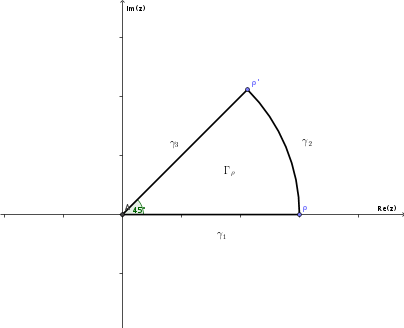
\includegraphics[scale=0.8]{2b.png}
\caption{A drawing of the contour $\Gamma_{\rho}$. $\gamma_1$ goes from $z = x=0$ to $z = x = \rho$. $\gamma_2$ goes from $z = \rho$ to $z = \rho e^{i\pi/4}$. $\gamma_3$ goes from $z = \rho e^{i\pi/4}$ and back to the origin.}
\end{figure}

We have the contour integral

$$
\tilde{I} = \int_{\Gamma_{\rho}} e^{iz^2}dz
$$

We want to check where $e^{iz^2}$ is analytic. We can do this by checking if $e^{iz^2}$ satisfy the Cauchy-Riemann conditions. We are going to use that $z = x+iy$:

$$
e^{iz^2} = e^{i(x + iy)^2} = e^{i(x^2 + 2xy -y^2)} = e^{-2xy}e^{x^2-y^2}
$$

We then use Euler's formula:

$$
= e^{-2xy}(\cos(x^2-y^2) + i\sin(x^2-y^2))
$$

We want this to be on the form $f(z) = u(x,y) + v(x,y)i$, where $u = Re(f)$ and $u = Im(f)$, so

$$
u(x,y) = e^{-2xy}\cos(x^2-y^2), \qquad v(x.y) = e^{-2xy}\sin(x^2-y^2)
$$

To check the Cauchy-Riemann conditions we need the derivatives of these functions:

$$
\frac{\partial u}{\partial x} = -2e^{-2xy}(x\sin(x^2-y^2) + y\cos(x^2 - y^2))
$$
$$
\frac{\partial u}{\partial y} = 2e^{-2xy}(y\sin(x^2-y^2) - x\cos(x^2 - y^2))
$$
$$
\frac{\partial v}{\partial x} = 2e^{-2xy}(x\cos(x^2-y^2) - y\sin(x^2 - y^2))
$$
$$
\frac{\partial u}{\partial y} = -2e^{-2xy}(x\sin(x^2-y^2) + y\cos(x^2 - y^2))
$$

From this we can quickly see that

$$
\frac{\partial u}{\partial x} = \frac{\partial v}{\partial y}, \qquad \frac{\partial u}{\partial y} = -\frac{\partial v}{\partial x}
$$

And so we see that $e^{iz^2}$ satisfy the Cauchy-Riemann conditions. Since we haven't explicitly chosen any specific $x,y$, we get that this is true independent of our choice of $x$ and $y$, meaning that for every $\rho$, $e^{iz^2}$ is analytic.\\

 The Cauchy Theorem says that if a function $f(z)$ is analytic inside and on a contour $\Gamma$ when

$$
\int_{\Gamma} f(z) dz = 0
$$

Since $e^{iz^2}$ is analytic on the entire complex plane, and therefor inside and on $\Gamma_{\rho}$:

$$
\underline{\underline{\tilde{I} = \int_{\Gamma_{\rho}} e^{iz^2}dz = 0}}
$$

\subsection*{c)}

The integral

$$
\tilde{I}_1 = \int_{\gamma_1} e^{iz^2} dz = \int_0^{\rho} e^{iz^2} dz
$$

is a integral over a line on the real axis, so to make this an integral of a real value we are going to do the trivial transformation:

$$
z = t, \qquad dz = dt
$$

And for the boundaries

$$
0 \rightarrow 0, \qquad \rho \rightarrow \rho
$$

So the integral becomes

$$
\int_{\gamma_1} e^{iz^2} dz = \int_0^{\rho} e^{it^2}dt
$$

This is closely connected to our original integral $I$. As $\rho$ becomes larger and larger, $\int_0^{\rho} e^{it^2}dt$ comes closer and closer to $I$. So:

\begin{equation}
I = \lim_{\rho \rightarrow \infty} \int_0^{\rho} e^{it^2}dt = \lim_{\rho \rightarrow \infty} \int_0^{\rho} e^{iz^2}dz
\label{eq:I1}
\end{equation}


\newpage
\subsection*{d)}

We have the integral

$$
\tilde{I}_ 3 = \int_{\gamma_3}e^{iz^2} dz = \int_{\rho e^{i\pi/4}}^0 e^{iz^2} dz 
$$

We have to make a change of variables. We are interested in getting simpler boundary conditions, so to 'guess' a way to make the $e^{i\pi/4}$ in the lower boundary disappear would give a good ansatz. So we are going to try:

$$
x = e^{-i\pi/4}z. \qquad dx = e^{-i\pi /4}dz
$$

The boundaries then becomes:

$$
z = \rho e^{i\pi/4} \rightarrow x = \rho, \qquad z = 0 \rightarrow x = 0
$$

We then look at the integrand:

$$
e^{iz^2} = e^{i(e^{i\pi/4}x)^2} = e^{ie^{i\pi/2}x^2} = e^{i\cdot ix^2} = e^{-x^2}
$$

This gives 

$$
\tilde{I}_3 = \int_{\rho}^0 e^{-x^2} e^{i\pi /4} dx = - \int_0^{\rho} e^{-x^2} e^{i\pi /4} dx
$$

We know that 

$$
e^{i\pi/4} =\frac{1+i}{\sqrt{2}}
$$

This gives us the final result:

\begin{equation}
\underline{\underline{\int_{\gamma_3}e^{iz^2} dz = -\frac{1+i}{\sqrt{2}}\int_0^{\rho}e^{-x^2}dx}}
\label{eq:I3}
\end{equation}



\subsection*{e)}
We have the integral

$$
\int_{\gamma_2}e^{iz^2} dz
$$

Where $\gamma = \rho e^{i\theta}$, with $0 \leq \theta \leq \pi/4$. From the $lemma$ in the exercise we know that

$$
|\int_0^{\rho} f(z) dz| \leq \int_0^{\rho} M(z) dz
$$

Where $M(z)$ is real, and $|f(z)| \leq M(z)$. We can start with by doing a transformation of our integral with $z = \rho e^{i\theta}$. We also need that

$$
\frac{dz}{d\theta} = i\rho e^{i\theta} \Rightarrow dz = i\rho e^{i\theta} d\theta
$$

Giving us that:

$$
\big| \int_{\gamma_2}e^{iz^2} dz \big| = \big|\int_0^{\pi/4} e^{i\rho^2 e^{2i\theta}} i\rho e^{i\theta} d\theta \big|
$$

Using Euler's formula:

$$
= \big|\int_0^{\pi/4} e^{i\rho^2 \cos(2\theta)}e^{-\rho^2 \sin(2\theta)} i\rho e^{i\theta} d\theta \big|
$$

We can try to eliminate some terms by using the generalized triangular inequality:

$$
\big|\int_0^{\pi/4} e^{i\rho^2 \cos(2\theta)}e^{-\rho^2 \sin(2\theta)} i\rho e^{i\theta} d\theta \big| \leq \int_0^{\pi/4} |e^{i\rho^2 \cos(2\theta)}||e^{-\rho^2 \sin(2\theta)}|\underbrace{|i|}_{=1}\underbrace{|e^{i\theta}|}_{=1}\rho d\theta
$$

We see that $e^{i\rho^2 \cos(2\theta)}$ is a rotation, meaning that $|e^{i\rho^2 \cos(2\theta)}| = 1$. We are here moving from a complex to a real function, meaning that we can imply the lemma from the exercise(I do not think this lemma is necessary here, because of the absolute values, meaning that the inequality below instead becomes an equality). So we get

$$
\int_0^{\pi/4} |e^{i\rho^2 \cos(2\theta)}||e^{-\rho^2 \sin(2\theta)}|\rho d\theta \leq \int_0^{\pi/4} |e^{-\rho^2 \sin(2\theta)}|\rho d\theta
$$

We now make an other change of variables:

$$
2\theta = \alpha, \qquad d\alpha = \frac{1}{2} d\theta, \qquad 0 \leq \alpha \leq \pi/2
$$

And since $e^{-\rho^2 \sin(2\theta)}$ is a real, positive quantity we get $|e^{-\rho^2 \sin(2\theta)}| = e^{-\rho^2 \sin(2\theta)}$. Combining these we get 

$$
\int_0^{\pi/4} |e^{-\rho^2 \sin(2\theta)}|\rho d\theta = \frac{1}{2}\int_0^{\pi/2} e^{-\rho^2 \sin(\alpha)}\rho d\alpha
$$

And we can now look closer at $\sin \alpha$. As hinted in the exercise, the line connection the two end points are less than $\sin \alpha$. We need to find that line. A straight line is given as:

$$
y(\alpha) - y_0 = a(\alpha - \alpha_0)
$$

First, for $\alpha = 0$ we have $\sin \alpha = 0$, so $x_0 = y_0 = 0$. Meaning:

$$
y = a\alpha
$$

To find $\alpha$ we look at the end point. We see that for $\alpha = \pi/2 \Rightarrow \sin\alpha = 1$, and find 

$$
1 = a\frac{\pi}{2} \Rightarrow a = \frac{2}{\pi}
$$ 

So the straight line connection the end points are given as

$$
y(\alpha) = \frac{2}{\pi}\alpha
$$

So from the hint we get that:

\begin{equation}
\sin \alpha \geq \frac{2\alpha}{\pi}
\label{eq:sinStraight}
\end{equation}

From above we had that 

$$
\big| \int_{\gamma_2}e^{iz^2} dz \big| \leq \frac{1}{2}\int_0^{\pi/2} e^{-\rho^2 \sin(\alpha)}\rho d\alpha
$$

We can use \eqref{eq:sinStraight} and see that this implies 

$$
\frac{1}{2}\int_0^{\pi/2} e^{-\rho^2 \sin(\alpha)}\rho d\alpha \leq \frac{1}{2}\int_0^{\pi/2} e^{-2\rho^2 \alpha/\pi}\rho d\alpha
$$

The last expression is an integral we can solve. This gives us:

$$
\frac{1}{2}\int_0^{\pi/2} e^{-2\rho^2 \alpha/\pi}\rho d\alpha = \frac{\pi}{4\rho} - \frac{\pi e^{-\alpha^2}}{4\rho}
$$

We see that $\frac{\pi e^{-\alpha^2}}{4\rho}$ is a positive, real number, meaning 

$$
\frac{\pi}{4\rho} - \frac{\pi e^{-\alpha^2}}{4\rho} \leq  \frac{\pi}{4\rho}
$$

And we get the final result:

\begin{equation}
\underline{\underline{\big| \int_{\gamma_2}e^{iz^2} dz \big| \leq \frac{\pi}{4\rho}}}
\label{eq:I2}
\end{equation}



\subsection*{f)}

We can now use all the above to find the integral $I$. We know that

$$
\tilde{I} = \tilde{I}_1 + \tilde{I}_2 + \tilde{I}_3 = 0
$$

We are interested in the case where $\rho$ goes to infinity. We are going to look at all the terms of the expression one by one, and see how they behave as $\rho$ goes to infinity.\\

$\underline{\mathbf{\tilde{I}}}$:\\

$\tilde{I} = 0$ independently of $\rho$, so
\begin{equation}
\lim_{\rho \rightarrow \infty} \tilde{I} = 0
\label{eq:IrhoInf}
\end{equation}\\

$\underline{\mathbf{\tilde{I}_1}}$:\\

We saw from \eqref{eq:I1} that

\begin{equation}
\lim_{\rho \rightarrow \infty} \tilde{I}_1 = \lim_{\rho \rightarrow \infty} \int_0^{\rho} e^{it^2} dt = I
\label{eq:I1rhoInf}
\end{equation}\\

$\underline{\mathbf{\tilde{I}_2}}$:\\

We found that \eqref{eq:I2}

$$
\bigg|\int_{\gamma_2}e^{iz^2}dz \bigg| \leq \frac{\pi}{4\rho}
$$

We can look at this upper bound. It is easy to see that

$$
\lim_{\rho\rightarrow \infty} \frac{\pi}{4\rho} = 0
$$
So we get that

$$
\lim_{\rho \rightarrow \infty } \bigg|\int_{\gamma_2}e^{iz^2}dz \bigg| \leq 0
$$

But since $\big|\int_{\gamma_2}e^{iz^2}dz \big|$ has to be positive, we get that

$$
\lim_{\rho \rightarrow \infty } \bigg|\int_{\gamma_2}e^{iz^2}dz \bigg| = 0
$$

If the length of the integral is zero, then the integral has to be zero, so:

\begin{equation}
\lim_{\rho \rightarrow \infty} \tilde{I}_2 = \lim_{\rho \rightarrow \infty}  \int_{\gamma_2}e^{iz^2}dz = 0
\label{I2rhoInf}
\end{equation}\\

$\underline{\mathbf{\tilde{I}_3}}$:\\

For the last integral we have that 

$$
\lim_{\rho \rightarrow \infty}  \int_{\gamma_3}e^{iz^2}dz = \lim_{\rho \rightarrow \infty} -\frac{1+i}{\sqrt{2}}  \int_0^{\rho}e^{-t^2}dt 
$$

We can look at the last part of that integral:

$$
\lim_{\rho \rightarrow \infty} \int_0^{\rho}e^{-t^2}dt  = \int_0^{\infty}e^{-t^2}dt
$$

This is a know integral we can look up in Rottman, where we find this to equal $\frac{\sqrt{\pi}}{2}$. So:

\begin{equation}
\lim_{\rho \rightarrow \infty} \tilde{I}_3 = \lim_{\rho \rightarrow \infty} \int_{\gamma_3}e^{iz^2}dz = \lim_{\rho \rightarrow \infty} -\frac{1+i}{\sqrt{2}}  \int_0^{\rho}e^{-t^2}dt = -\frac{1+i}{\sqrt{2}} \frac{\sqrt{\pi}}{2}
\label{I3rhoinf}
\end{equation}\\

We can now use all this to find the original integral $I$.

$$
\lim_{\rho \rightarrow \infty} \tilde{I} = \lim_{\rho \rightarrow \infty} \tilde{I}_1 + \lim_{\rho \rightarrow \infty} \tilde{I}_2 + \lim_{\rho \rightarrow \infty} \tilde{I}_3 = 0
$$

and by using \eqref{eq:I1rhoInf}, \eqref{I2rhoInf} and \eqref{I3rhoinf} we find that

$$
\lim_{\rho \rightarrow \infty} \tilde{I} = I + 0 - \frac{1+i}{\sqrt{2}} \frac{\sqrt{\pi}}{2} = 0
$$

This gives us the final result:

$$
I = \int_0^{\infty}e^{it^2}dt =\underline{\underline{\left(\frac{1}{2} +\frac{i}{2}\right) \sqrt{\frac{\pi}{2}}}}
$$\\

We can now use this to evaluate some integrals. We are going to start by noting that:

$$
\int_0^{\infty}e^{it^2}dt = \int_0^{\infty} \cos(t^2) + i\sin(t^2)dt
$$

This means that $I$ has a real and an imaginary part. We can quickly see from this that:

$$
\int_0^{\infty} \cos(t^2)dt = Re(\int_0^{\infty}e^{it^2}dt) = Re\left(\left(\frac{1}{2} +\frac{i}{2}\right) \sqrt{\frac{\pi}{2}}\right) = \underline{\underline{\frac{1}{2}\sqrt{\frac{\pi}{2}}}}
$$

And

$$
\int_0^{\infty} \sin(t^2)dt = Im(\int_0^{\infty}e^{it^2}dt) = Im\left(\left(\frac{1}{2} +\frac{i}{2}\right) \sqrt{\frac{\pi}{2}}\right) = \underline{\underline{\frac{1}{2}\sqrt{\frac{\pi}{2}}}}
$$

We get that the two integrals are equivalent. 


\newpage
\section*{3)}
\subsection*{a)}

Fermat's principle is given by

\begin{equation}
P = \int_A^B n(r) ds
\end{equation}

For polar coordinates the line element $ds$ is given as 

$$
ds = \sqrt{dr^2 + r^2d\theta^2}
$$

Giving us the path

$$
P = \int_A^B n(r) \sqrt{dr^2 + r^2d\theta^2}
$$

Now, we have two alternatives, we can either put out $dr$ or $d\theta$ from the square root, giving us two different integrals:

\begin{equation}
P_1 = \int_A^B n(r)\sqrt{1 + r^2 \left(\frac{d\theta}{dr}\right)^2} dr
\label{eq:p1}
\end{equation}



and

\begin{equation}
P_2 = \int_A^B n(r)\sqrt{r^2 +  \left(\frac{dr}{d\theta}\right)^2} d\theta
\label{eq:p2}
\end{equation}



We are interested in the minima of these paths. This is a problem in calculus of variation, which we know how to solve. We can find the shortest path by the using Euler-Lagrange equation. If we look at $P_1$ we see that it has no explicit dependence on $\theta$. Meaning that if we write the Euler-Lagrange equation for $P_1$:

$$
\frac{d}{dr}\frac{\partial L}{\partial \theta'} - \frac{\partial L}{\partial \theta} = 0
$$ 

Where $L = n(r)\sqrt{1 + r^2 \left(\frac{d\theta}{dr}\right)^2}$.\\

We can see that the term $\frac{\partial L}{\partial \theta}$ disappears($\theta$ is a \textit{cyclic} variable). This gives us a much easier equation to solve, as the problem reduces from a second order, to a first order differential equation:

\begin{equation}
\frac{d}{dr}\frac{\partial L}{\partial \theta'} = 0 \Leftrightarrow \frac{\partial L}{\partial \theta'} = C
\label{eq:lagrange}
\end{equation}

Where $C$ is some constant.\\

This is now the case for $P_2$, which is explicitly dependent on $\theta$, $\theta'$ and $r$. So $P_1$ is the best choice.

\newpage
\subsection*{b)}

We are now going to start to minimize the path of $P_1$ \eqref{eq:p1}. As mentioned above this means we have to solve the Euler-Lagrange equation, which we showed reduces \eqref{eq:lagrange} to

$$
\frac{\partial L}{\partial \theta'} = C
$$

Where

$$
L = n(r)\sqrt{1 + r^2 \left(\frac{d\theta}{dr}\right)^2}
$$

Taking the partial differentiation we get that:

$$
\frac{\partial L}{\partial \theta'} = n(r) \frac{r^2\theta'}{\sqrt{1 + r^2\theta'^2}} = C
$$

where $\theta' = \frac{d\theta}{dr}$. To solve this differential equation we need to clean up the expression, to make it possible to separate the variables. We start by taking the square of both sides:

$$
\Rightarrow n^2(r)\frac{r^4 \theta'^2}{1+r^2\theta'^2} = C^2 = D
$$

Then interchanging $D$ and $1+r^2\theta'^2$, and isolation $r^2\theta'^2$:

$$
\frac{n^2(r)}{D}r^4\theta'^2 = 1 + r^2\theta'^2
$$

$$
r^2\theta'^2\left(\frac{n^2(r)}{D}r^2 - 1\right) = 1
$$

Then moving $r^2\theta'^2$ to the RHS:

$$
\Rightarrow r^2\frac{n^2(r)}{D} - 1 = \frac{1}{r^2}\frac{1}{\theta'^2}
$$

We can see that 

$$
\frac{1}{\theta'^2} = \left(\frac{d\theta}{dr}\right)^{-2} = \left(\frac{dr}{d\theta}\right)^2
$$

So we get:

$$
\frac{1}{r^2}\left(\frac{dr}{d\theta}\right)^2 = r^2\frac{n^2(r)}{D} -1
$$

We now need to get rid of the constant $D$. We know that at the distance $d$ is the closes point in the path to the point $\mathcal{O}$, and thus we have that $\frac{\partial L}{\partial \theta} = 0$. We insert this in to the above expression to find $D$:


$$
\left(\frac{dr}{d\theta}\right)^2_{r = d} = 0 = d^2\frac{n^2(d)}{D} -1
$$

$$
\Rightarrow d^2\frac{n^2(d)}{D} = 1 \Leftrightarrow D = d^2 n^2(d)
$$

We can now eliminate $D$, and find that:

\begin{equation}
\underline{\underline{\frac{1}{r^2}\left(\frac{dr}{d\theta}\right)^2 = \frac{r^2}{d^2}\frac{n^2(r)}{n^2(d)} -1}}
\label{eq:sepDiff}
\end{equation}


\subsection*{c)}

Now we have a separable DE \eqref{eq:sepDiff}. We are going to use that the refractive index is given as 

\begin{equation}
n(r) = \sqrt{1 + \frac{\kappa^2}{r^2}}
\label{eq:refIndex}
\end{equation}

This also gives us the refractive index at $d$ is given as

$$
n(d) = \sqrt{1 + \frac{\kappa^2}{d^2}}
$$

If we insert this into \eqref{eq:sepDiff} we get that 

$$
\frac{1}{r^2}\left(\frac{dr}{d\theta}\right)^2 = \frac{r^2}{d^2}\frac{1 + \frac{\kappa^2}{r^2}}{1 + \frac{\kappa^2}{d^2}} -1
$$
$$
= \frac{r^2 + \kappa^2}{d^2+\kappa^2} - 1 = \frac{r^2 + \kappa^2}{d^2+\kappa^2} - \frac{d^2+\kappa^2}{d^2+\kappa^2} = \frac{r^2 -d^2}{d^2 +\kappa^2}
$$
So

$$
\left(\frac{dr}{d\theta}\right)^2 = r^2\frac{r^2 -d^2}{d^2 +\kappa^2}
$$


We are interested inn an expression for $\theta$, so we can write the above as:

\begin{equation}
d\theta = \frac{1}{r}\left(\frac{r^2 -d^2}{d^2 +\kappa^2}\right)^{-1/2}dr
\end{equation}


We are interested in finding how much the light is refracted when it moves from far way, gets refracted inside the medium, comes to a distance $d$ from $\mathcal{O}$ then move far way.

\begin{figure}[H]
\centering
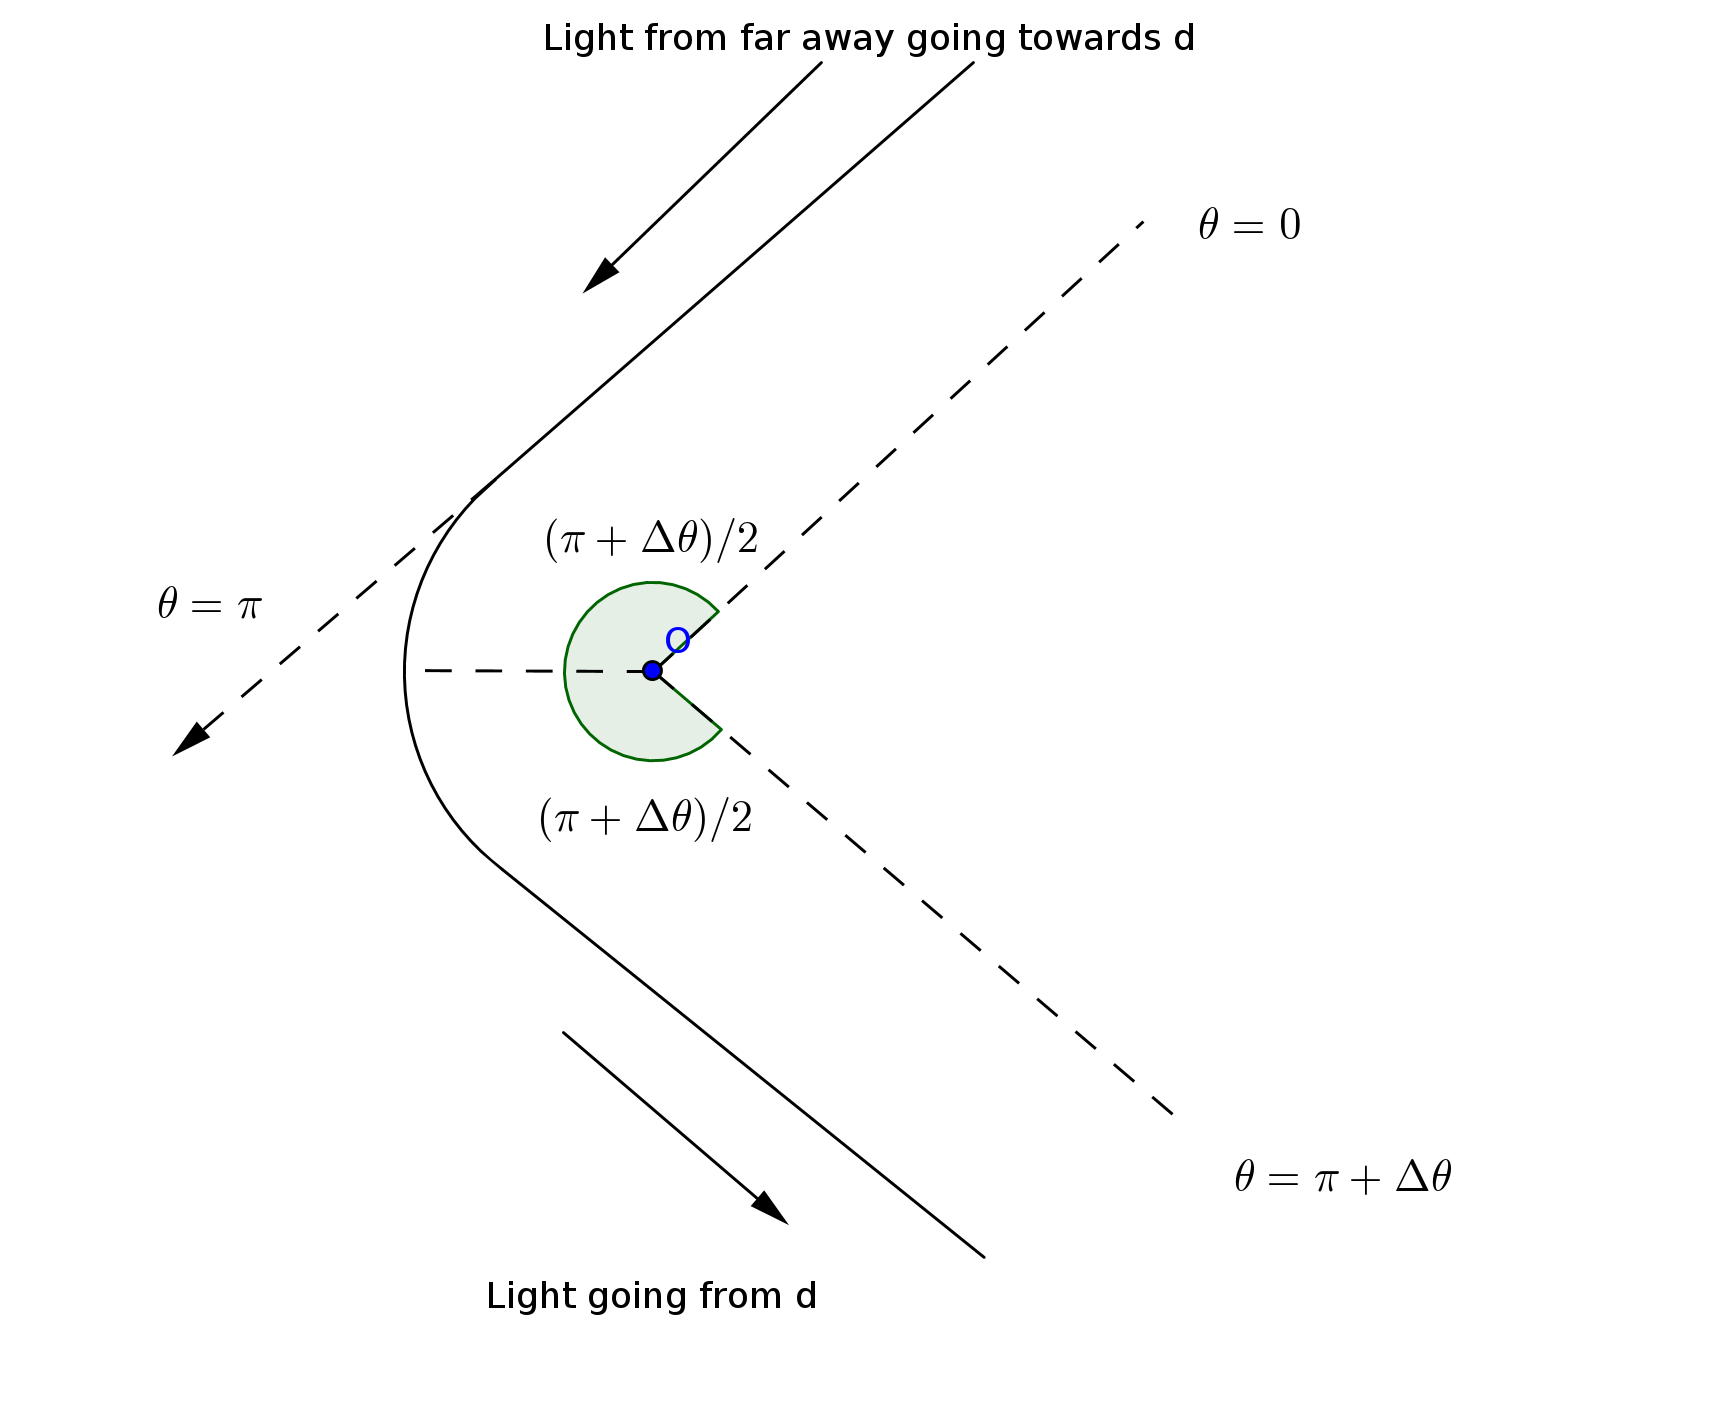
\includegraphics[scale=0.4]{3c.png}
\caption{A crude drawing of the light moving from far away to d, then away from $\mathcal{O}$. We can see that the light deflects the same amount on both the way in and the way out. This figure and the method used below is heavily inspired by the AST1100 lecture notes on gravitational lensing.}
\end{figure}

Since the refractive index is only dependent on the distance from $\mathcal{O}$ the deflection angle will be the same as the light moves in, as when it moves out. This means that we only have to calculate the deflection angle for the light moving from $r = d$ to $r = \infty$($d$ being the nearest point to $\mathcal{O}$, and I am going to set 'far away' as meaning $r\rightarrow \infty$). The angle is also defined such that a non-deflected light beam would have a $\Delta \theta = 0$, there is an other alternative where a non-deflected beam would have $\Delta \theta = \pi$. \\

As seen in the picture the angular deflection from $r = d$ to $r = \infty$ is $(\pi + \Delta\theta) - (\pi/2 +\Delta\theta/2)$. So:

$$
\Delta\theta_{d\rightarrow \infty}=\int_{\pi/2 +\Delta\theta/2}^{\pi + \Delta\theta} d\theta = \frac{\pi}{2} + \frac{\Delta \theta}{2} = \int_d^{\infty} \frac{1}{r}\left(\frac{r^2 -d^2}{d^2 +\kappa^2}\right)^{-1/2}dr
$$

$$
= \sqrt{d^2 +\kappa^2}\int_d^{\infty} \frac{1}{r\sqrt{r^2 - d^2}}dr
$$

We are going to use a change of variable:

$$
r = d \cosh x
$$

We find the Jacobi factor:

$$
\frac{dr}{dx} = d\sinh x \Leftrightarrow dr = d\sinh(x) dx
$$

Since we are changing variables we have to change the boundaries:

$$
\lim_{r\rightarrow \infty}\cosh^{-1} \frac{r}{d} = \infty, \qquad \cosh^{-1}\frac{d}{d} = 0
$$

We then get the integral:

$$
\Delta\theta_{d\rightarrow \infty} = \sqrt{d^2 +\kappa^2}\int_0^{\infty} \frac{d\sinh x}{d\cosh x\sqrt{d^2\cosh^2 x - d^2}}dx
$$

$$
= \frac{\sqrt{d^2 +\kappa^2}}{d}\int_0^{\infty} \tanh x \frac{1}{\sqrt{\cosh^2 x - 1}}dx
$$

We know that $\cosh^2 x - 1 = \sinh^2 x$, so since $\tanh x = \frac{\sinh x}{\cosh x}$ we get that:

$$
\frac{\pi}{2} + \frac{\Delta \theta}{2} = \frac{\sqrt{d^2 +\kappa^2}}{d}\int_0^{\infty} \frac{1}{\cosh x}dx
$$

Using Rottman we find that this is:

$$
= \frac{\sqrt{d^2 +\kappa^2}}{d} (\arcsin(\tanh x)) \bigg|_0^{\infty}
$$

$$
= \frac{\sqrt{d^2 +\kappa^2}}{d} \left(\frac{\pi}{2} - 0\right) = \frac{\sqrt{d^2 +\kappa^2}}{d} \frac{\pi}{2}
$$

This gives us that 
$$
\frac{\pi}{2} + \frac{\Delta \theta}{2} = \frac{\sqrt{d^2 +\kappa^2}}{d} \frac{\pi}{2}
$$


Which gives us the expression for the angle deflection:

$$
\Delta \theta = \theta_{end} - \theta_{start} = \underline{\underline{\pi \left(\frac{\sqrt{d^2 +\kappa^2}}{d} - 1\right)}}
$$

An easy check is to check the boundary where $d \rightarrow \infty$:

$$
\Delta \theta_{\infty} = \lim_{d\rightarrow \infty}  \pi \left(\frac{\sqrt{d^2 +\kappa^2}}{d} - 1\right) = 0
$$

As we would expect.\\

 As mentioned above, if we use the definition that for a non-deflected beam $\Delta \theta = \pi$ we'll get an other answer. We would instead get the answer:

$$
\Delta \theta = \pi\frac{\sqrt{d^2 + \kappa^2}}{d}
$$

I think that the way I have defined a non-deflected beam is more intuitive, but I mention this just to show the other alternative.




\end{document}


